% 01.tex
\documentclass[platex,dvipdfmx,draft]{jsreport}

\usepackage{graphicx}
\graphicspath{{./images}{../images}}
\usepackage{pdfpages}
\usepackage{tikz}
\usepackage{xcolor}
\definecolor{UD_GREEN}{HTML}{03af7a}
\usepackage{bm}
\usepackage[left=30truemm]{geometry}
\usepackage{amsmath,amssymb}
\numberwithin{equation}{section}
% \subfiletrue
\begin{document}

\chapter{序論}


\section{背景}

  %% 目次
\subsection{フォトニック結晶}

\begin{figure}[htbp]
  \centering
  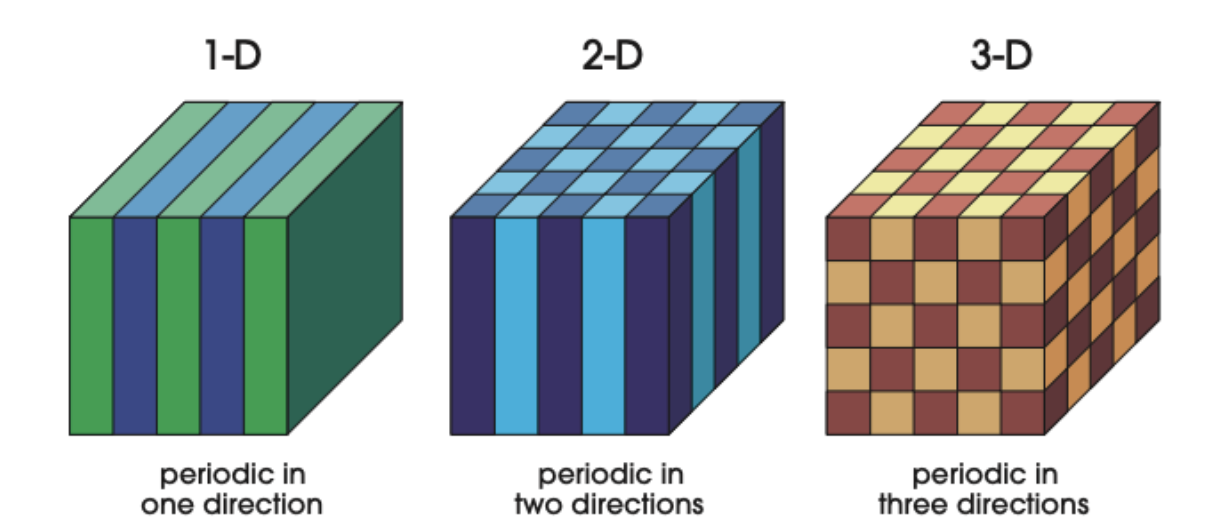
\includegraphics[width=0.9\linewidth]{crystals.png}
  \caption{フォトニック結晶の構造}
  \label{fig:photonic_crystal}
\end{figure}


フォトニック結晶は、1987年に、E.Yablonovitchが提案した概念であり、屈折率の異なる材質を周期的に配置した誘電体である。特に、フォトニックバンドギャップと呼ばれる、波数ベクトルに関わらず結晶中にどのモードも存在できないような周波数ギャップを持つように設計されたフォトニック結晶は、特定の方向への光の伝播を制御することが可能となる。
完全なフォトニックバンドギャップを有する構造には、一次元では多層膜、二次元では三角格子、三次元ではダイヤモンド構造などが知られている。


\subsection{MIT Photonic Bands}

MIT Photonic Bands (MPB) は、マサチューセッツ工科大学のSteven G. Johnsonによって開発された、ソフトウェアパッケージである。周期的誘電体構造における固有状態やバンド構造などの計算の機能を持っており、フォトニック結晶の研究に適している。また、フォトニック結晶に限らず、導波路や共振器システムなどの光学分野において活用することができる。

MPBは、誘電体構造の計算には時間領域法ではなく周波数領域法を用いている。これによって周波数と電磁モードを同時に取得を可能としている。従来の周波数領域固有ソルバーでは、目的の固有状態まで多数のバンドを計算する必要があったが、ターゲット固有ソルバーという手法を用いることでバンドギャップを直接解決し計算量と記憶容量のコストの削減を図っている。


技術的には、PythonやSchemeといった汎用のプログラミング言語から制御できるほか、HDF5形式での電場状態の出力に対応しているなど、他のプログラムと入出力において互換性を持たせるように設計された。libctl(Steven G. Johnsonによる開発)によって柔軟なインターフェースが提供され、手軽に条件を指定して計算することができる。またフーリエ変換にはFFTW (こちらもSteven G. Johnsonらによる開発)を用いている。現在もMITライセンスの元でオープンソースでメンテナンスされている。


\section{目的}
本研究では、フォトニック結晶の基礎的な構造である3次元フォトニック結晶に着目し、フォトニックバンドギャップを最大化する構造を見つけることを目的とする。MPBを用いたプログラムによって結晶のパラメータや誘電率などを変化させ、パラメータとバンドギャップの関連性を調べる。

\end{document}
